\chapter{Terminals for Data Processing} 
\label{terminals}

The {\bf Terminal} or {\bf Platform} in this report refers to the machine or computer (hardware) which handles the processing of the raw measurements acquired from the sensors, the visualisation of the data received, in addition to the transmission and reception of the information from one geographical location to another through electromagnetic waves. Multiple types of terminals were considered and the factors which were accounted for were:

\begin{enumerate}
	\item Processing Power
	\item Operating System
	\item Price
	\item Power Consumption
	\item Wireless Capabilities
	\item Number of Input/Output Ports
\end{enumerate} 

\section{Operating System}
\label{os}

Of all the factors mentioned above, the OS for the Terminal is the most important and deserves a section of its own for further discussion. The OS must be fully capable of running the software required for data processing, data visualisation, virtual network computing (VNC) server hosting, and wireless transmission. Consequently, the OS determines which Terminal should be chosen as some platforms are designed based on a specific OS.  

Based on the above criteria, Linux was chosen for this project due to the open source nature of the OS. Many software programs and applications required for the functionality specified, such as the ones mentioned in Section \ref{software}, are readily available without cost from the Linux software database. Despite being an open source technology, security is not a concern but on the contrary, a significant advantage \cite{linuxadvantagedisadvantage}. By releasing the source code of the OS to the general public, security experts from various backgrounds and fields are able to identify major security flaws in the system \cite{linuxadvantagedisadvantage}. This allows for the swift resolution of such breaches by developers around the world, making security issues nullified as soon as they are found. Unlike proprietary OS such as Windows, the international community of developers are the ones who maintain the system for Linux, rather than a fixed number of employees working in specific locations around the world.  

Nevertheless, one substantial problem with Linux OS is drivers for new hardware components \cite{linuxadvantagedisadvantage}. However, due to the lower level nature of this project, drivers can be developed and so does not pose a major threat. Other drivers required for microcontrollers such as the Arduino Uno/Arduino Pro Mini for analogue to digital conversion are readily available and hence, does not pose a major threat.  

One such platform which runs on a Linux kernel is the Rasberry Pi 3. The Linux distribution which was suggested by default for this miniaturised computer is the Raspbian Jessie, which is the Raspberry Pi derivative of the long standing Debian distribution. Section \ref{rpi} has been dedicated to further analyse the Raspberry Pi 3 Model B used for this project. 

Having a platform that runs on a Linux kernel provides the significant advantage of the ease of migration. As the project is a pilot study in wireless vital signs monitoring systems, there is a foreseeable need to continuously upgrade the platforms in terms of hardware capabilities to accommodate other important features. As long as the Linux kernel is used, it is not difficult to migrate to another more powerful Linux-based platform as the applications database and drivers available do not greatly differ for specific Linux distributions. \\


of all these, the OS is the most important - deserves a section of its own for discussion
very important - terminal is chosen based on this

Raspbian Jessie - Linux kernel - open source - more software and support available 

- ease of migrating to other platforms - as long as the kernel remains the same 

- windows considered -but proprietary - software will be expensive - issues if no support - limited support - need for payment

linux provides 
\cite{linuxwindows}

\section{Raspberry Pi 3 Model B}
\label{rpi}

Based on the criteria set out in Section \ref{os}, the Raspberry Pi 3 Model B loaded with a Raspbian Jessie OS is chosen as the platform or terminal for the project, henceforth referred to as the \textbf{Raspberry Pi}.

\begin{figure}[H]
	\centering
	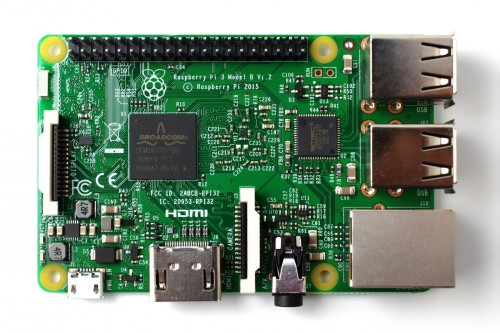
\includegraphics[width=0.7\linewidth]{rpi3.jpg}
	\caption{Raspberry Pi 3 Model B \cite{rpi3pic}}
	\label{rpi3pic}
\end{figure}


\cite{rpi3mb}

The specifications of the Raspberry Pi 3 Model B are as follows \cite{rpi3mb}: 
\begin{itemize}
	\item 1.2GHz 64-bit quad-core ARMv8 CPU
	\item 802.11n Wireless LAN
	\item Bluetooth 4.1
	\item Bluetooth Low Energy (BLE)
	\item 1GB RAM
	\item 4 USB ports
	\item 40 GPIO pins
	\item Full HDMI port
	\item Ethernet port
	\item Combined 3.5mm audio jack and composite video
	\item Camera interface (CSI)
	\item Display interface (DSI)
	\item Micro SD card slot (now push-pull rather than push-push)
	\item VideoCore IV 3D graphics core
\end{itemize}

The Raspberry Pi's CPU is capable of running different types of Linux-based OS, in particular, ARM Linux distributions. Examples of such OS are Raspbian and Ubuntu Mate, whereas an instance of a non-Linux-based OS is the Windows 10 IoT Core. As discussed in Section \ref{os}, it is preferable to use the Raspbian Jessie as it is designed specifically for the Raspberry Pi. 

In terms of connectivity, the Raspberry Pi leaves little to be desired with an integrated 802.11n Wireless LAN. This inbuilt WiFi adapter provides the needed wireless interface for the WVSMS and lays the foundation of the project back end design. An Ethernet port is also available as a contingency for reliable operation. 

The 4 USB ports and 40 GPIO pins allow the sensors to be connected to the Terminal. However, it is important to note that all GPIO pins on the Raspberry Pi are only for digital input and output. Due to the absence of the analog-to-digital converters, there is a need to implement an interface for the Sensors, which provide signals in analog form. This is done using the Arduino Uno/Arduino Pro Mini as seen in Section \ref{arduino}. 

The full HDMI port and VideoCore IV 3D graphics core provides the graphic processing power required to render the images when data is visualised and displays it to a monitor. 

Based on the criteria laid out in Section \ref{terminals}, the Raspberry Pi provides the necessary processing power, operating system, power consumption, wireless capabilities, and input/output ports at a reasonable price. 

The schematic design of the Raspberry Pi 3 Model B can be found in Appendix \ref{rpi3bschematic}.

\cite{rpi3hardware}


\subsection{Raspbian Jessie}

Raspbian Jessie is 
\cite{rpi3raspbian}
https://www.raspbian.org/

Installation instructions can be found in Appendix \ref{appraspbianjessie}


Version:May 2016
Release date:2016-05-27
Kernel version:4.4


\subsection{Portable Power Supply for the Raspberry Pi 3 Model B}
\cite{rpi3faqs}

The Raspberry Pi is powered using a 5V micro-USB power supply\cite{rpi3faqs}. The current drawn by the Raspberry Pi is variable and depends on the applications running in addition to the current drawn by peripheral devices which are connected. Typically, the Raspberry Pi 3 Model B current requirements range from 1.2A to 2.5A \cite{rpi3faqs}. 

Buck - 9V

\section{Intel Nuc}

